%  LaTeX support: latex@mdpi.com 
%  For support, please attach all files needed for compiling as well as the log file, and specify your operating system, LaTeX version, and LaTeX editor.

%=================================================================
\documentclass[engproc,conferenceproceedings,submit,pdftex,moreauthors]{Definitions/mdpi} 

%--------------------
% Class Options:
%--------------------
%----------
% journal
%----------
% Choose between the following MDPI journals:
% acoustics, actuators, addictions, admsci, adolescents, aerobiology, aerospace, agriculture, agriengineering, agrochemicals, agronomy, ai, air, algorithms, allergies, alloys, analytica, analytics, anatomia, animals, antibiotics, antibodies, antioxidants, applbiosci, appliedchem, appliedmath, applmech, applmicrobiol, applnano, applsci, aquacj, architecture, arm, arthropoda, arts, asc, asi, astronomy, atmosphere, atoms, audiolres, automation, axioms, bacteria, batteries, bdcc, behavsci, beverages, biochem, bioengineering, biologics, biology, biomass, biomechanics, biomed, biomedicines, biomedinformatics, biomimetics, biomolecules, biophysica, biosensors, biotech, birds, bloods, blsf, brainsci, breath, buildings, businesses, cancers, carbon, cardiogenetics, catalysts, cells, ceramics, challenges, chemengineering, chemistry, chemosensors, chemproc, children, chips, cimb, civileng, cleantechnol, climate, clinpract, clockssleep, cmd, coasts, coatings, colloids, colorants, commodities, compounds, computation, computers, condensedmatter, conservation, constrmater, cosmetics, covid, crops, cryptography, crystals, csmf, ctn, curroncol, cyber, dairy, data, ddc, dentistry, dermato, dermatopathology, designs, devices, diabetology, diagnostics, dietetics, digital, disabilities, diseases, diversity, dna, drones, dynamics, earth, ebj, ecologies, econometrics, economies, education, ejihpe, electricity, electrochem, electronicmat, electronics, encyclopedia, endocrines, energies, eng, engproc, entomology, entropy, environments, environsciproc, epidemiologia, epigenomes, est, fermentation, fibers, fintech, fire, fishes, fluids, foods, forecasting, forensicsci, forests, foundations, fractalfract, fuels, future, futureinternet, futurepharmacol, futurephys, futuretransp, galaxies, games, gases, gastroent, gastrointestdisord, gels, genealogy, genes, geographies, geohazards, geomatics, geosciences, geotechnics, geriatrics, grasses, gucdd, hazardousmatters, healthcare, hearts, hemato, hematolrep, heritage, higheredu, highthroughput, histories, horticulturae, hospitals, humanities, humans, hydrobiology, hydrogen, hydrology, hygiene, idr, ijerph, ijfs, ijgi, ijms, ijns, ijpb, ijtm, ijtpp, ime, immuno, informatics, information, infrastructures, inorganics, insects, instruments, inventions, iot, j, jal, jcdd, jcm, jcp, jcs, jcto, jdb, jeta, jfb, jfmk, jimaging, jintelligence, jlpea, jmmp, jmp, jmse, jne, jnt, jof, joitmc, jor, journalmedia, jox, jpm, jrfm, jsan, jtaer, jvd, jzbg, kidneydial, kinasesphosphatases, knowledge, land, languages, laws, life, liquids, literature, livers, logics, logistics, lubricants, lymphatics, machines, macromol, magnetism, magnetochemistry, make, marinedrugs, materials, materproc, mathematics, mca, measurements, medicina, medicines, medsci, membranes, merits, metabolites, metals, meteorology, methane, metrology, micro, microarrays, microbiolres, micromachines, microorganisms, microplastics, minerals, mining, modelling, molbank, molecules, mps, msf, mti, muscles, nanoenergyadv, nanomanufacturing,\gdef\@continuouspages{yes}} nanomaterials, ncrna, ndt, network, neuroglia, neurolint, neurosci, nitrogen, notspecified, %%nri, nursrep, nutraceuticals, nutrients, obesities, oceans, ohbm, onco, %oncopathology, optics, oral, organics, organoids, osteology, oxygen, parasites, parasitologia, particles, pathogens, pathophysiology, pediatrrep, pharmaceuticals, pharmaceutics, pharmacoepidemiology,\gdef\@ISSN{2813-0618}\gdef\@continuous pharmacy, philosophies, photochem, photonics, phycology, physchem, physics, physiologia, plants, plasma, platforms, pollutants, polymers, polysaccharides, poultry, powders, preprints, proceedings, processes, prosthesis, proteomes, psf, psych, psychiatryint, psychoactives, publications, quantumrep, quaternary, qubs, radiation, reactions, receptors, recycling, regeneration, religions, remotesensing, reports, reprodmed, resources, rheumato, risks, robotics, ruminants, safety, sci, scipharm, sclerosis, seeds, sensors, separations, sexes, signals, sinusitis, skins, smartcities, sna, societies, socsci, software, soilsystems, solar, solids, spectroscj, sports, standards, stats, std, stresses, surfaces, surgeries, suschem, sustainability, symmetry, synbio, systems, targets, taxonomy, technologies, telecom, test, textiles, thalassrep, thermo, tomography, tourismhosp, toxics, toxins, transplantology, transportation, traumacare, traumas, tropicalmed, universe, urbansci, uro, vaccines, vehicles, venereology, vetsci, vibration, virtualworlds, viruses, vision, waste, water, wem, wevj, wind, women, world, youth, zoonoticdis 
% For posting an early version of this manuscript as a preprint, you may use "preprints" as the journal. Changing "submit" to "accept" before posting will remove line numbers.

%---------
% article
%---------
% The default type of manuscript is "article", but can be replaced by: 
% abstract, addendum, article, book, bookreview, briefreport, casereport, comment, commentary, communication, conferenceproceedings, correction, conferencereport, entry, expressionofconcern, extendedabstract, datadescriptor, editorial, essay, erratum, hypothesis, interestingimage, obituary, opinion, projectreport, reply, retraction, review, perspective, protocol, shortnote, studyprotocol, systematicreview, supfile, technicalnote, viewpoint, guidelines, registeredreport, tutorial
% supfile = supplementary materials

%----------
% submit
%----------
% The class option "submit" will be changed to "accept" by the Editorial Office when the paper is accepted. This will only make changes to the frontpage (e.g., the logo of the journal will get visible), the headings, and the copyright information. Also, line numbering will be removed. Journal info and pagination for accepted papers will also be assigned by the Editorial Office.

%------------------
% moreauthors
%------------------
% If there is only one author the class option oneauthor should be used. Otherwise use the class option moreauthors.

%---------
% pdftex
%---------
% The option pdftex is for use with pdfLaTeX. Remove "pdftex" for (1) compiling with LaTeX & dvi2pdf (if eps figures are used) or for (2) compiling with XeLaTeX.

\usepackage{caption}
\usepackage{subcaption}
%=================================================================
% MDPI internal commands - do not modify
\firstpage{1} 
\makeatletter 
\setcounter{page}{\@firstpage} 
\makeatother
\pubvolume{1}
\issuenum{1}
\articlenumber{0}
\pubyear{2023}
\copyrightyear{2023}
%\externaleditor{Academic Editor: Firstname Lastname}
\datereceived{ } 
\daterevised{ } % Comment out if no revised date
\dateaccepted{ } 
\datepublished{ } 
%\datecorrected{} % For corrected papers: "Corrected: XXX" date in the original paper.
%\dateretracted{} % For corrected papers: "Retracted: XXX" date in the original paper.
\hreflink{https://doi.org/} % If needed use \linebreak
%\doinum{}
%\pdfoutput=1 % Uncommented for upload to arXiv.org

%=================================================================
% Add packages and commands here. The following packages are loaded in our class file: fontenc, inputenc, calc, indentfirst, fancyhdr, graphicx, epstopdf, lastpage, ifthen, float, amsmath, amssymb, lineno, setspace, enumitem, mathpazo, booktabs, titlesec, etoolbox, tabto, xcolor, colortbl, soul, multirow, microtype, tikz, totcount, changepage, attrib, upgreek, array, tabularx, pbox, ragged2e, tocloft, marginnote, marginfix, enotez, amsthm, natbib, hyperref, cleveref, scrextend, url, geometry, newfloat, caption, draftwatermark, seqsplit
% cleveref: load \crefname definitions after \begin{document}

%=================================================================
% Please use the following mathematics environments: Theorem, Lemma, Corollary, Proposition, Characterization, Property, Problem, Example, ExamplesandDefinitions, Hypothesis, Remark, Definition, Notation, Assumption
%% For proofs, please use the proof environment (the amsthm package is loaded by the MDPI class).

%=================================================================
% Full title of the paper (Capitalized)
% Author Orchid ID: enter ID or remove command

\Title{Enhanced Pedestrian Dead Reckoning Sensor Fusion for Firefighting }

% MDPI internal command: Title for citation in the left column
\TitleCitation{Enhanced Pedestrian Dead Reckoning Sensor Fusion for Firefighting }

\newcommand{\orcidauthorA}{0009-0000-9900-4172} % Add \orcidA{} behind the author's name
\newcommand{\orcidauthorB}{0000-0003-4499-5639} % Add \orcidB{} behind the author's name

% Authors, for the paper (add full first names)
\Author{Tobias Augustin $^{1}$*, Daniel Ossmann $^{1}$\orcidB{} }

%\longauthorlist{yes}

% MDPI internal command: Authors, for metadata in PDF
\AuthorNames{Tobias Augustin, Daniel Ossmann}

% MDPI internal command: Authors, for citation in the left column
\AuthorCitation{Augustin, T.; Ossmann, D.}
% If this is a Chicago style journal: Lastname, Firstname, Firstname Lastname, and Firstname Lastname.

% Affiliations / Addresses (Add [1] after \address if there is only one affiliation.)
\address{%
	$^{1}$ \quad Munich University of Applied Sciences HM \\}

% Contact information of the corresponding author
\corres{Correspondence: tobias.augustin@hm.edu}

% Current address and/or shared authorship
%\firstnote{Current address: Affiliation 3.} 
%\secondnote{These authors contributed equally to this work.}
% The commands \thirdnote{} till \eighthnote{} are available for further notes

%\simplesumm{} % Simple summary

%\conference{} % An extended version of a conference paper

% Abstract (Do not insert blank lines, i.e. \\) 
\abstract{Knowing the exact position of firefighters in a building during an indoor firefighting operation is critical to improving the efficiency and safety of firefighters. For the estimation of an individual's  position in indoor or Global Positioning System (GPS) denied environments commonly Pedestriasn Dead Reckoning (PDR) is used. PDR tries to estimate the required position via sensors without	external references, for example using accelerometers and gyroscopes. One of the most common techniques of PDR is step-detection. Applications like firefighting, however, involve more dynamic movements like crouching. Thus, the accuracy of a step-detection algorithm is reduced dramatically. Therefore, this paper presents a novel PDR algorithm that augments the conventional PDR technique with a tracking camera. The position estimates of a zero-crossing step-detection algorithm and the tracking camera estimates are fused via a Kalman filter. A system prototype, designed for algorithm validation, is presented in detail. The experimental  results confirm that enhancing the system with a secondary sensor leads to a substantial   increase in the position estimation accuracy also for dynamic crouching maneuvers compared to conventional step-detection algorithms.}


% Keywords
\keyword{Step Detection; Firefighting; Kalman Filter} 

% The fields PACS, MSC, and JEL may be left empty or commented out if not applicable
%\PACS{J0101}
%\MSC{}
%\JEL{}

%%%%%%%%%%%%%%%%%%%%%%%%%%%%%%%%%%%%%%%%%%
% Only for the journal Diversity
%\LSID{\url{http://}}

%%%%%%%%%%%%%%%%%%%%%%%%%%%%%%%%%%%%%%%%%%
% Only for the journal Applied Sciences
%\featuredapplication{Authors are encouraged to provide a concise description of the specific application or a potential application of the work. This section is not mandatory.}
%%%%%%%%%%%%%%%%%%%%%%%%%%%%%%%%%%%%%%%%%%

%%%%%%%%%%%%%%%%%%%%%%%%%%%%%%%%%%%%%%%%%%
% Only for the journal Data
%\dataset{DOI number or link to the deposited data set if the data set is published separately. If the data set shall be published as a supplement to this paper, this field will be filled by the journal editors. In this case, please submit the data set as a supplement.}
%\datasetlicense{License under which the data set is made available (CC0, CC-BY, CC-BY-SA, CC-BY-NC, etc.)}

%%%%%%%%%%%%%%%%%%%%%%%%%%%%%%%%%%%%%%%%%%
% Only for the journal Toxins
%\keycontribution{The breakthroughs or highlights of the manuscript. Authors can write one or two sentences to describe the most important part of the paper.}

%%%%%%%%%%%%%%%%%%%%%%%%%%%%%%%%%%%%%%%%%%
% Only for the journal Encyclopedia
%\encyclopediadef{For entry manuscripts only: please provide a brief overview of the entry title instead of an abstract.}

%%%%%%%%%%%%%%%%%%%%%%%%%%%%%%%%%%%%%%%%%%
% Only for the journal Advances in Respiratory Medicine
%\addhighlights{yes}
%\renewcommand{\addhighlights}{%

%\noindent This is an obligatory section in “Advances in Respiratory Medicine”, whose goal is to increase the discoverability and readability of the article via search engines and other scholars. Highlights should not be a copy of the abstract, but a simple text allowing the reader to quickly and simplified find out what the article is about and what can be cited from it. Each of these parts should be devoted up to 2~bullet points.\vspace{3pt}\\
%\textbf{What are the main findings?}
% \begin{itemize}[labelsep=2.5mm,topsep=-3pt]
% \item First bullet.
% \item Second bullet.
% \end{itemize}\vspace{3pt}
%\textbf{What is the implication of the main finding?}
% \begin{itemize}[labelsep=2.5mm,topsep=-3pt]
% \item First bullet.
% \item Second bullet.
% \end{itemize}
%}

%%%%%%%%%%%%%%%%%%%%%%%%%%%%%%%%%%%%%%%%%%
\begin{document}

%%%%%%%%%%%%%%%%%%%%%%%%%%%%%%%%%%%%%%%%%%

\section{Introduction}

While safety standards in firefighting are continuously improving, indoor operations in burning buildings still present a dangerous task for firefighters. At least 240 injuries and 10 deaths involving firefighters conducting firefighting operations in buildings were reported in the United States in 2022 \cite{atemschutzunfalle.eu2023}. To improve safety while performing such a dangerous task, knowing the exact position of firefighters in indoor environments can shorten rescue time of injured personnel or help firefighters avoiding dangerous situations. To determine the position of a person in indoor or GPS-denied environments, a technique called Pedestrian Dead Reckoning (PDR) is used. It relies on sensors such as accelerometers, gyroscopes, and magnetometers integrated into wearable devices, smartphones or smartwatches. By continuously tracking a pedestrian's step counts, stride length, and heading changes, PDR algorithms can calculate their relative displacement from a known starting point. Other means of PDR include simultaneous locating and mapping (SLAM)\cite{lu2019}, magnetic field mapping \cite{wang2016} or magnetic triangulation \cite{arumugam2020}.

For an application in firefighting operations, many of the aforementioned PDR methods are not feasible. While radio tracking \cite{cong2023} or magnetic mapping \cite{wang2016} produce accurate results in indoor environments, they are technologies that have to be installed before use. It may be possible to achieve this for some large buildings, however it would not be feasible to do for every building in an area where a fire might occur. For tracking firefighters in any indoor environment, a stand-alone, body-worn device is required. Stand-alone PDR systems often rely on a form of step-detection \cite{hou2021}. Algorithms based on step-detection can estimate an accurate position mainly  during walking. Movements occurring in a firefighting application, however, also include more dynamic activities like crouching. Those movements are hard to detect by standard step-detection algorithms. Thus, a secondary sensor measuring position or velocity is necessary to improve accuracy in those scenarios. A common sensor chosen for this is a Light Detection and Ranging (LIDAR) sensor \cite{wang2016}. While this approach can yield good results in smoke-free environments, tests show that distance readings of LIDAR systems are heavily influenced by smoke particles and therefore are not usable in a firefighting environment.

Due to these shortcomings in PDR for firefighting application, in this paper  a novel approach for enhanced PDR is presented. The step-detection algorithm is extended with a stereo tracking camera as a secondary sensor. This tracking camera is able to visually determine velocity and position relative to a starting point, even is smoky scenarios. The camera providing position and velocity is combined with a step-detection algorithm providing position information. The gathered data is 
fused using a Kalman filter to robustly estimate the firefighters position. While in section 2 the fundamentals of the step-detection and the model for the Kalman filter is presented, in section 3 the overall PDR system setup including software and hardware components is described. Finally, section 4 discusses the results of a verification campaign in which position data from the proposed algorithm is compared to data generated by step-detection only.


%%%%%%%%%%%%%%%%%%%%%%%%%%%%%%%%%%%%%%%%%%
\section{Sensor-Data Processing Algorithms}
The PDR relies on an advanced sensor data fusion algorithm combining position data estimated by a step-detection algorithm and the velocity and position data estimates of a secondary sensor.

\subsection{Step-Length Estimation}\label{sub:stepD}
Step-detection describes the process of detecting and counting a persons steps by measuring and analysing the accelerations of a body-worn inertial measurement unit (IMU). The most common ways of step-detection utilize  the vertical acceleration signal and analyse the signal using peak-, zero-crossing or flat zone detection. A zero-crossing detection approach is chosen since flat zone detection only works for foot mounted sensors and peak-detection accuracy is dependent on a persons walking speed \cite{shin2007}. Zero-crossing detection analyses the characteristic shape of the vertical acceleration of a torso mounted sensor \cite{zhao2022}. To improve detection accuracy, the high-frequency content of the signal is filtered out using a lowpass filter. A straightforward implementation of a first order low pass filter is the so-called exponentially weighted moving average 
\begin{equation}
	y(k\Delta_T) = \alpha u(k\Delta_T) + (1-\alpha) y((k-1)\Delta_T), 
\end{equation} where $u(k\Delta_T)$ is the raw signal at time step $k\Delta_T$, and $y(k\Delta_T)$ and $y((k-1)\Delta_T)$ is the filtered signal of the current and the last time step, respectively  \cite{nistsematech2012}. The smoothing factor $\alpha$ lies between 0 and 1 and can be calculated as 
\begin{equation}
	\alpha = \frac{2\pi \Delta_T f_c}{2\pi \Delta_T f_c +1},
\end{equation} with $\Delta_T$ being the sampling time and $f_c$ being the required cut-off frequency.  For a step to be counted as complete, the filtered, vertical acceleration signal $a_z$ has to cross the zero line twice, once rising, i.e.,
\begin{equation}
	(a_{z} > 0) \wedge (a_{z} < 0)  %Größer Null etc.!!
\end{equation} 
and afterwards once falling, i.e.,
\begin{equation}
	(a_{z} < 0) \wedge (a_{z} > 0).  %Größer Null etc.!!
\end{equation} 
Only if these two conditions have been registered in the algorithm, a step can be finally counted.

Once  a step is registered as complete, the step length has to be added to the current estimated position in the direction of movement. To estimate the step-length $d$ a method  using the relation between hip acceleration and the length of a step following  \cite{weinberg2002} is applied, i.e.,
 \begin{equation}\label{eq:dist}
	d = \sqrt[4]{a_{\max}-a_{\min}} \, n \, c.
\end{equation}
In equation (\ref{eq:dist}) with $a_{\max}$ is the maximum possible acceleration during a single step and $A_{\min}$ the minimal possible acceleration during a step with $n$ being the number of steps taken and $c$ being a constant gain for unit conversion. This method produces accurate estimates with low computational effort compared to other algorithms \cite{petukhov2022, shin2007, zizzo2017}.
%\begin{figure}[h!]
%	\centering
%	\includegraphics[width=0.5\textwidth,height=5cm]{test.png}
%	\caption{Acceleration Signal during one step}
%\end{figure}



 
\subsection{Sensor-Data Fusion}
Sensor-data fusion describes the process of using multiple sensor outputs to estimate the state of a system. A common approach for sensor fusion complementary filtering, which combines high frequency data of one sensor, that fast but prone to drift, with low frequency data from another sensor, which stabilized the output signal.
In this paper we use the more advanced method of a Kalman filtering. The idea of the Kalman filter is to use an optimal recursive algorithm  for sensor-data fusion. The filter operates in two steps: the prediction step, where the system's state  is predicted using a prediction model, i.e., a mathematical model of the underlying dynamics; and the update step, \textcolor{red}{where measurements are used to correct the predicted state by computing the Kalman gain - Frage: stimmt das? wird das gain wirklich mit den measurements bestimmt? oder setzen sie das gain fest und es mischt die messungen zum modell?!}. This gain balances the model's predictions and the actual measurements \cite{chui2009}. The process continually refines the state estimate as new data becomes available, making it robust against noise and capable of handling real-time applications. The required prediction model is described by  the non-linear function $x((k+1)\,\Delta_T) = f(x(k\,\Delta_T),u(k\,\Delta_T))$. As underlying model in this paper we define for each of the three coordinate  axis the function 
\begin{equation}\label{eq:nl}
	f(x,u) = \begin{pmatrix}
		a \\
		a \Delta_T   \\
		v \, \Delta_T   + a \, \Delta_T^2  
		\end{pmatrix}
\end{equation}
with $a$ being the acceleration and $v$ being the velocity. The three elements of the vector in equation (\ref{eq:nl}) basically describe the estimates of the  acceleration, the velocity and the position.
Note that the dependency of the signals on time, i.e., on $k\Delta_T$, is omitted in equation (\ref{eq:nl}) for readability reasons.
 The measurement inputs are the acceleration $a$, velocity $v$ and position $x$ measurements for each of the three axes. By changing the covariance matrices of the Kalman filter, the accuracy of the predictions and measurement updates is tuned. \textcolor{red}{Hier braucht es ne Referenz zur Kalman filter literatur, sonst hängt das mit der Kovarianz in der Luft!!} \\

\textcolor{red}{Gleichung (6) ist noch nicht sauber; denn wir schreiben f(u,x), aber es is komplett unnklar was u und was x ist. Z.b. sehe ich keine position in gleichung 6 obwohl sie es so erwähnen. So wie es da steht sind v und a eher Eingängen und keine zustände. Und die Zustande sind dann halt jeweils das integral von der Eingängen auf der rechten Seite, tauchen aber nicht explizit in f() auf, das wäre also dann nur ein f(u). Ist das so gedacht? \\ Zudem ist mir nun nicht klar, was die Sensor fusion ist; kommt a und v aus unterschiedlicen sensoren? ich sehe nicht wo die potionsdaten von der step detection da eingehen. aber dasklär sich ws wenn ich weiß was u ist. }



%\begin{figure}[h!]
%	\centering
%	\includegraphics[width=\textwidth,height=7cm]{test.png}
%	\caption{Test}
%\end{figure}

% Description Experiment
\section{Enhanced Pedestriasn Dead Reckoning System}

% \begin{figure}[h!]
	% 	\centering
	% 	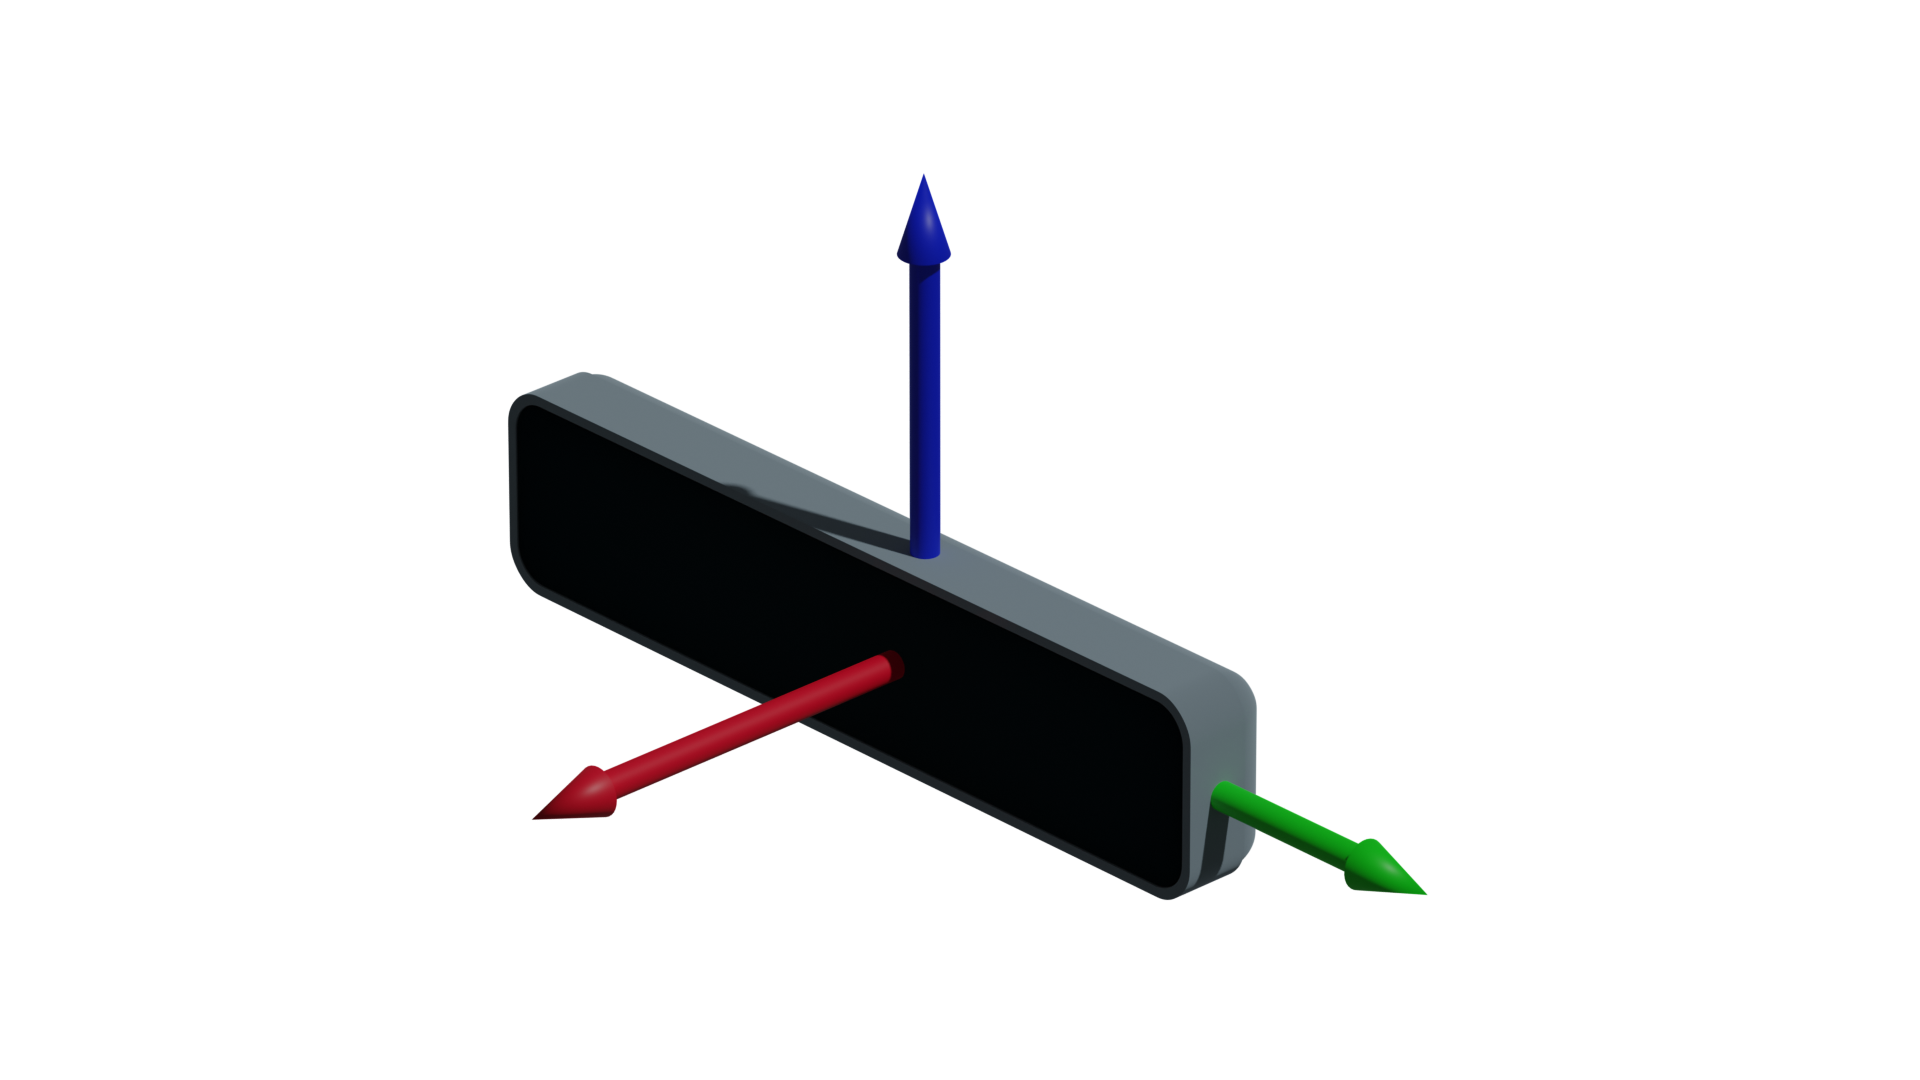
\includegraphics[width=0.7\textwidth]{realsense.png}
	% 	\caption{Realsense Tracking Camera with body coordinate system}
	% 	\label{fig:cmaera}
	% \end{figure}
	
 The step-detection uses a zero-crossing technique described in Section \ref{sub:stepD} enhanced with a threshold-crossing detection to improve the algorithm's robustness: The vertical acceleration signal is filtered with an exponentially weighted moving average lowpass filter (LPF) to remove the high frequency parts of the signal that occur during movement. Since the frequency range of normal human walking is in the range of 1 to 5\,Hz, the bandwidth of the LPF is specified at 10\,Hz. Figure \ref{fig:AccelWalk} shows the unfiltered and filtered acceleration signal. \textcolor{red}{ich würde versuchen eide graphen in ein diagramm zu tun, so kann man den unterschied nur erahnen} The signal is then analyzed by the step-detection algorithm: First the acceleration has to pass a set negative threshold $\tau_{\min}$. After $\tau_{\min} = -1.5$\,m/s$^2$ is passed, a zero crossing has to be detected, and the acceleration has to rise above the positive threshold $\tau_{\max}$. If $\tau_{\max} = 1.5\,\mathrm{m/s^2}$ is passed and another zero-crossing is detected, the step is counted as completed. If the step is not completed in a specified time or the negative threshold is not passed the step-detection logic is reset and no step is counted. 
% Figure \ref{fig:accelerationWalking} shows the vertical acceleration during walking and the points detected by the algorithm. 
%A schematic representation of the step-detection algorithm can be seen in Figure \ref{fig:algorithmStedDetect}
\begin{figure}[h!]
	\centering
	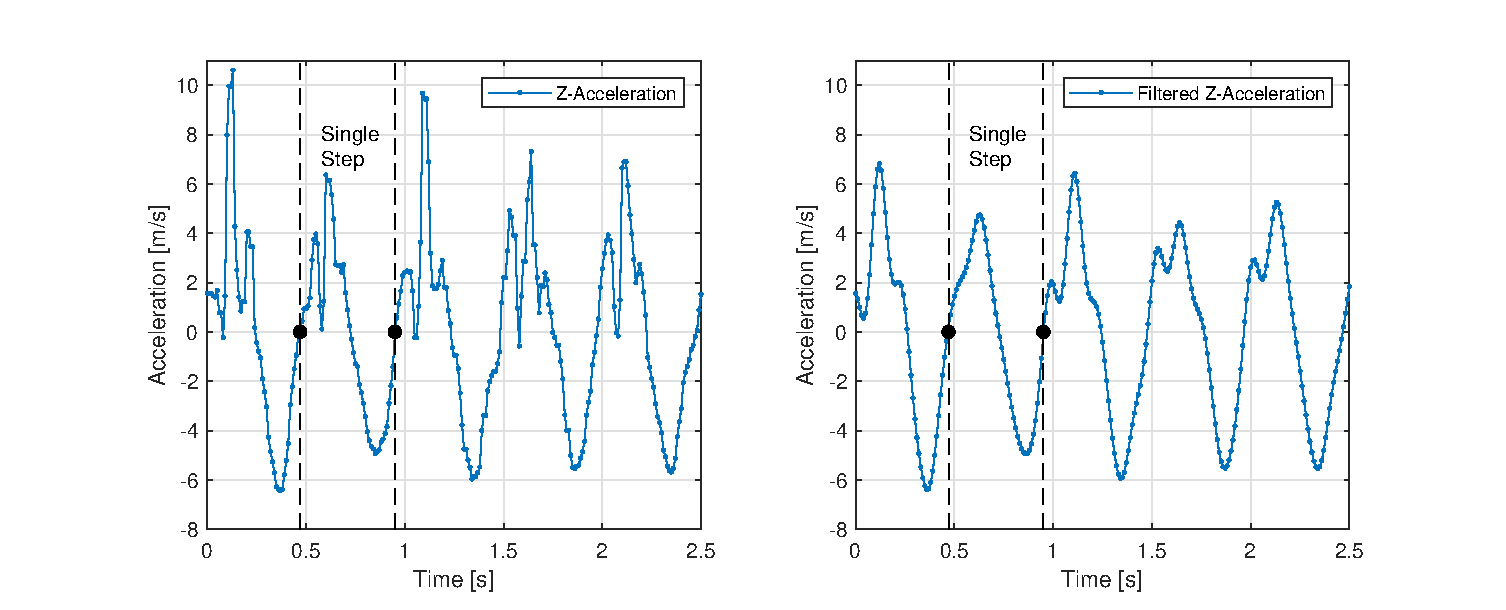
\includegraphics[width=\textwidth]{WalkAcceleration.eps}
	\caption{Vertical acceleration during walking, raw data on the left and filtered data on the right.}
	\label{fig:AccelWalk}
\end{figure}


%\begin{figure}[h!]
%	\centering
%	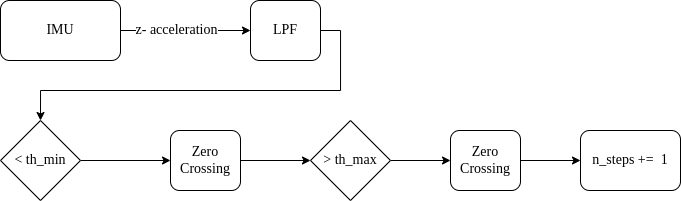
\includegraphics[width=\textwidth]{algorithmStepDetect.png}
%	
%	\caption{Vertical acceleration during walking}
%	\label{fig:algorithmStedDetect}
%\end{figure}

After a step is detected, the length of the step is added to the last known position in the direction of movement which is determined by the heading angle measured by the IMU. The step-length is estimated with the method described in section \ref{sub:stepD}. It is assumed, that because of limited field of view and restriction of movement by gear during an indoor operation with self-contained breathing apparatus (scba), firefighters will in most cases move in the direction their body is pointed. Since the IMU is mounted on the air tank of the firefighter, the orientation of the IMU equals the direction of movement. To describe the position in a global reference frame, the coordinate origin of the global reference frame $n$ is defined when the device is initialized: The initial heading direction defines the x-Axis. The z-Axis is set to be the Axis normal to the ground plane. As the secondary sensor a stereo tracking camera is chosen. Stereo tracking cameras work similarly to the human eye: The device has two calibrated cameras that are placed with a distance to each other and are horizontally aligned. By measuring the displacement of a tracked object between the two cameras, the distance to the object can be calculated. 
Doing this for multiple objects and repeating this process every frame, the position and average velocity can be calculated. 
%Figure \ref{fig:cmaera} shows the two aligned cameras as well as the cameras body coordinate frame.
Some camera models also use an infrared projected grid of dots to determine depth of the surrounding environment and can create a 3D profile.


The position calculated by the step-detection as well as the position and velocity measured by the tracking camera then get fused in a Kalman filter which is implemented using the Matlab Tracking Kalman Filter library.
The position estimates from the tracking camera and the step detection have to be weighted. The weighting scheme is determined by: Time since last step was detected. It is assumed that the accuracy of the estimated position by the step-detection algorithm deteriorates with time if no succeeding step is detected. Three conditions are proposed: the time passed since the last detection event $t_{\text{step}} < 0.5\mathrm{s}$, $5\mathrm{s} \leq t_{\text{step}} < 3\mathrm{s}$ or $t_{\text{step}} \geq 3\mathrm{s}$. Tracking Confidence of the tracking camera. The tracking camera is able to calculate and return a confidence value of the tracking results. The tracking confidence returned by the camera can reach four cases from zero to three, where three is the highest confidence and zero the lowest.

%\begin{itemize}
%	\item Time since last step was detected. It is assumed that the accuracy of the estimated position by the step-detection algorithm deteriorates with time if no succeeding step is detected. Three conditions are proposed: the time passed since the last detection event $t_{step} < 0.5\mathrm{s}$, $5\mathrm{s} \leq t_{step} < 3\mathrm{s}$ or $t_{step} \geq 3\mathrm{s}$.\\
%	
%	\item Tracking Confidence of the tracking camera. The tracking camera is able to calculate and return a confidence value of the tracking results. The tracking confidence returned by the camera can reach four cases from zero to three, where three is the highest confidence and zero the lowest.
%\end{itemize}



To combine the two measurements and take the confidence markers into account, a weighting scheme is proposed. The weighting scheme includes nine cases. This approach was influenced by the method presented in \cite{caron2006}. Goal of this approach is to weight and combine the inputs to achieve the best measurement.  If the quality of both markers is bad, the step detection gets highly favoured, since it provides stable results during walking, even in zero visibility environments. If the tracking confidence is high, the camera measurements get slightly favoured. This is because in theory the tracking cameras results will more accurate since it produces continuos position updates and can track the position regardless of the type of movement. %Figure \ref{fig:confidence} shows a graphical representation of the weighting scheme. 
The combination of the measurements is performed before they are used in the Kalman Filter. With a combination factor  $a$ the weighted measurement input for the x- and y-position
\begin{equation}
	\begin{pmatrix}
		x_k\\
		y_k
	\end{pmatrix} =
	\begin{pmatrix}
		a\cdot x_{\text{step}} + (1-a)\cdot x_{\text{camera}}\\
		a\cdot y_{\text{step}} + (1-a)\cdot y_{\text{camera}}
	\end{pmatrix}
\end{equation}  
is calculated with $x_{\text{step}}$ and $y_{\text{step}}$ being the position estimates produced by the step-detection and $x_{\text{camera}}$ and $y_{\text{camera}}$ being the position estimate from the tracking camera. Since the z-position has only one measurement input, no weighting is performed.
%\begin{figure}[h!]
%	\centering
%	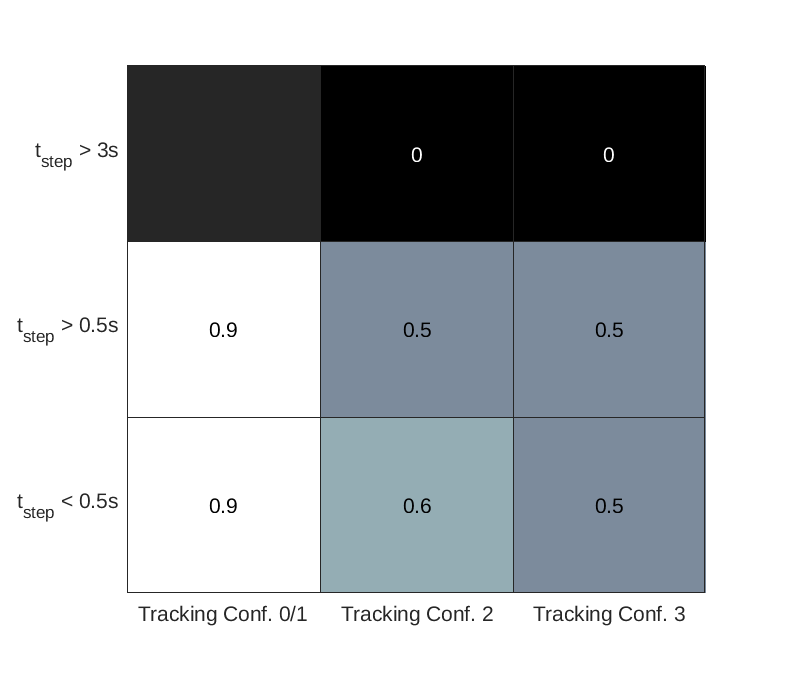
\includegraphics[width=0.5\textwidth]{measurementQuality.eps}
%	\caption{$a$ value for measurements of different quality}
%	\label{fig:confidence}}{Nenner}
%	
%\end{figure}

\subsection{Sensor Assembly}
 % Sensor assembly
 
The IMU used  is the Bosch Sensortech BNO055 MEMS absolute orientation sensor. The device measures acceleration in three axes and provides absolute heading data by measuring the earths magnetic field and fusing gyroscope and Magnetometer data. 
  
The secondary sensor chosen is a RealSense T265 stereo tracking camera. Its main advantage is the on-chip, online data processing, meaning that no other means of interpreting the data is necessary and the velocity and position data can be directly used for the sensor data fusion. By using parts of the infrared spectrum the camera also can produce accurate tracking results in environments with bad lighting.
  
For experimental verification of the system, a wearable sensor assembly is designed. Both sensors are mounted to the backplate of a self-contained breathing apparatus. This design is chosen to imitate a application in a firefighting setting, where the sensors would be placed on the pressurized air tank of the scba. For this a 3D printed spacer is designed to mount the sensors at the right distance. A weight is added to represent the scba air tank. The camera and IMU are protected from damage by a custom enclosure.  Figure \ref{fig:Assembly} shows the experimental setup.

\begin{figure}
	\centering
	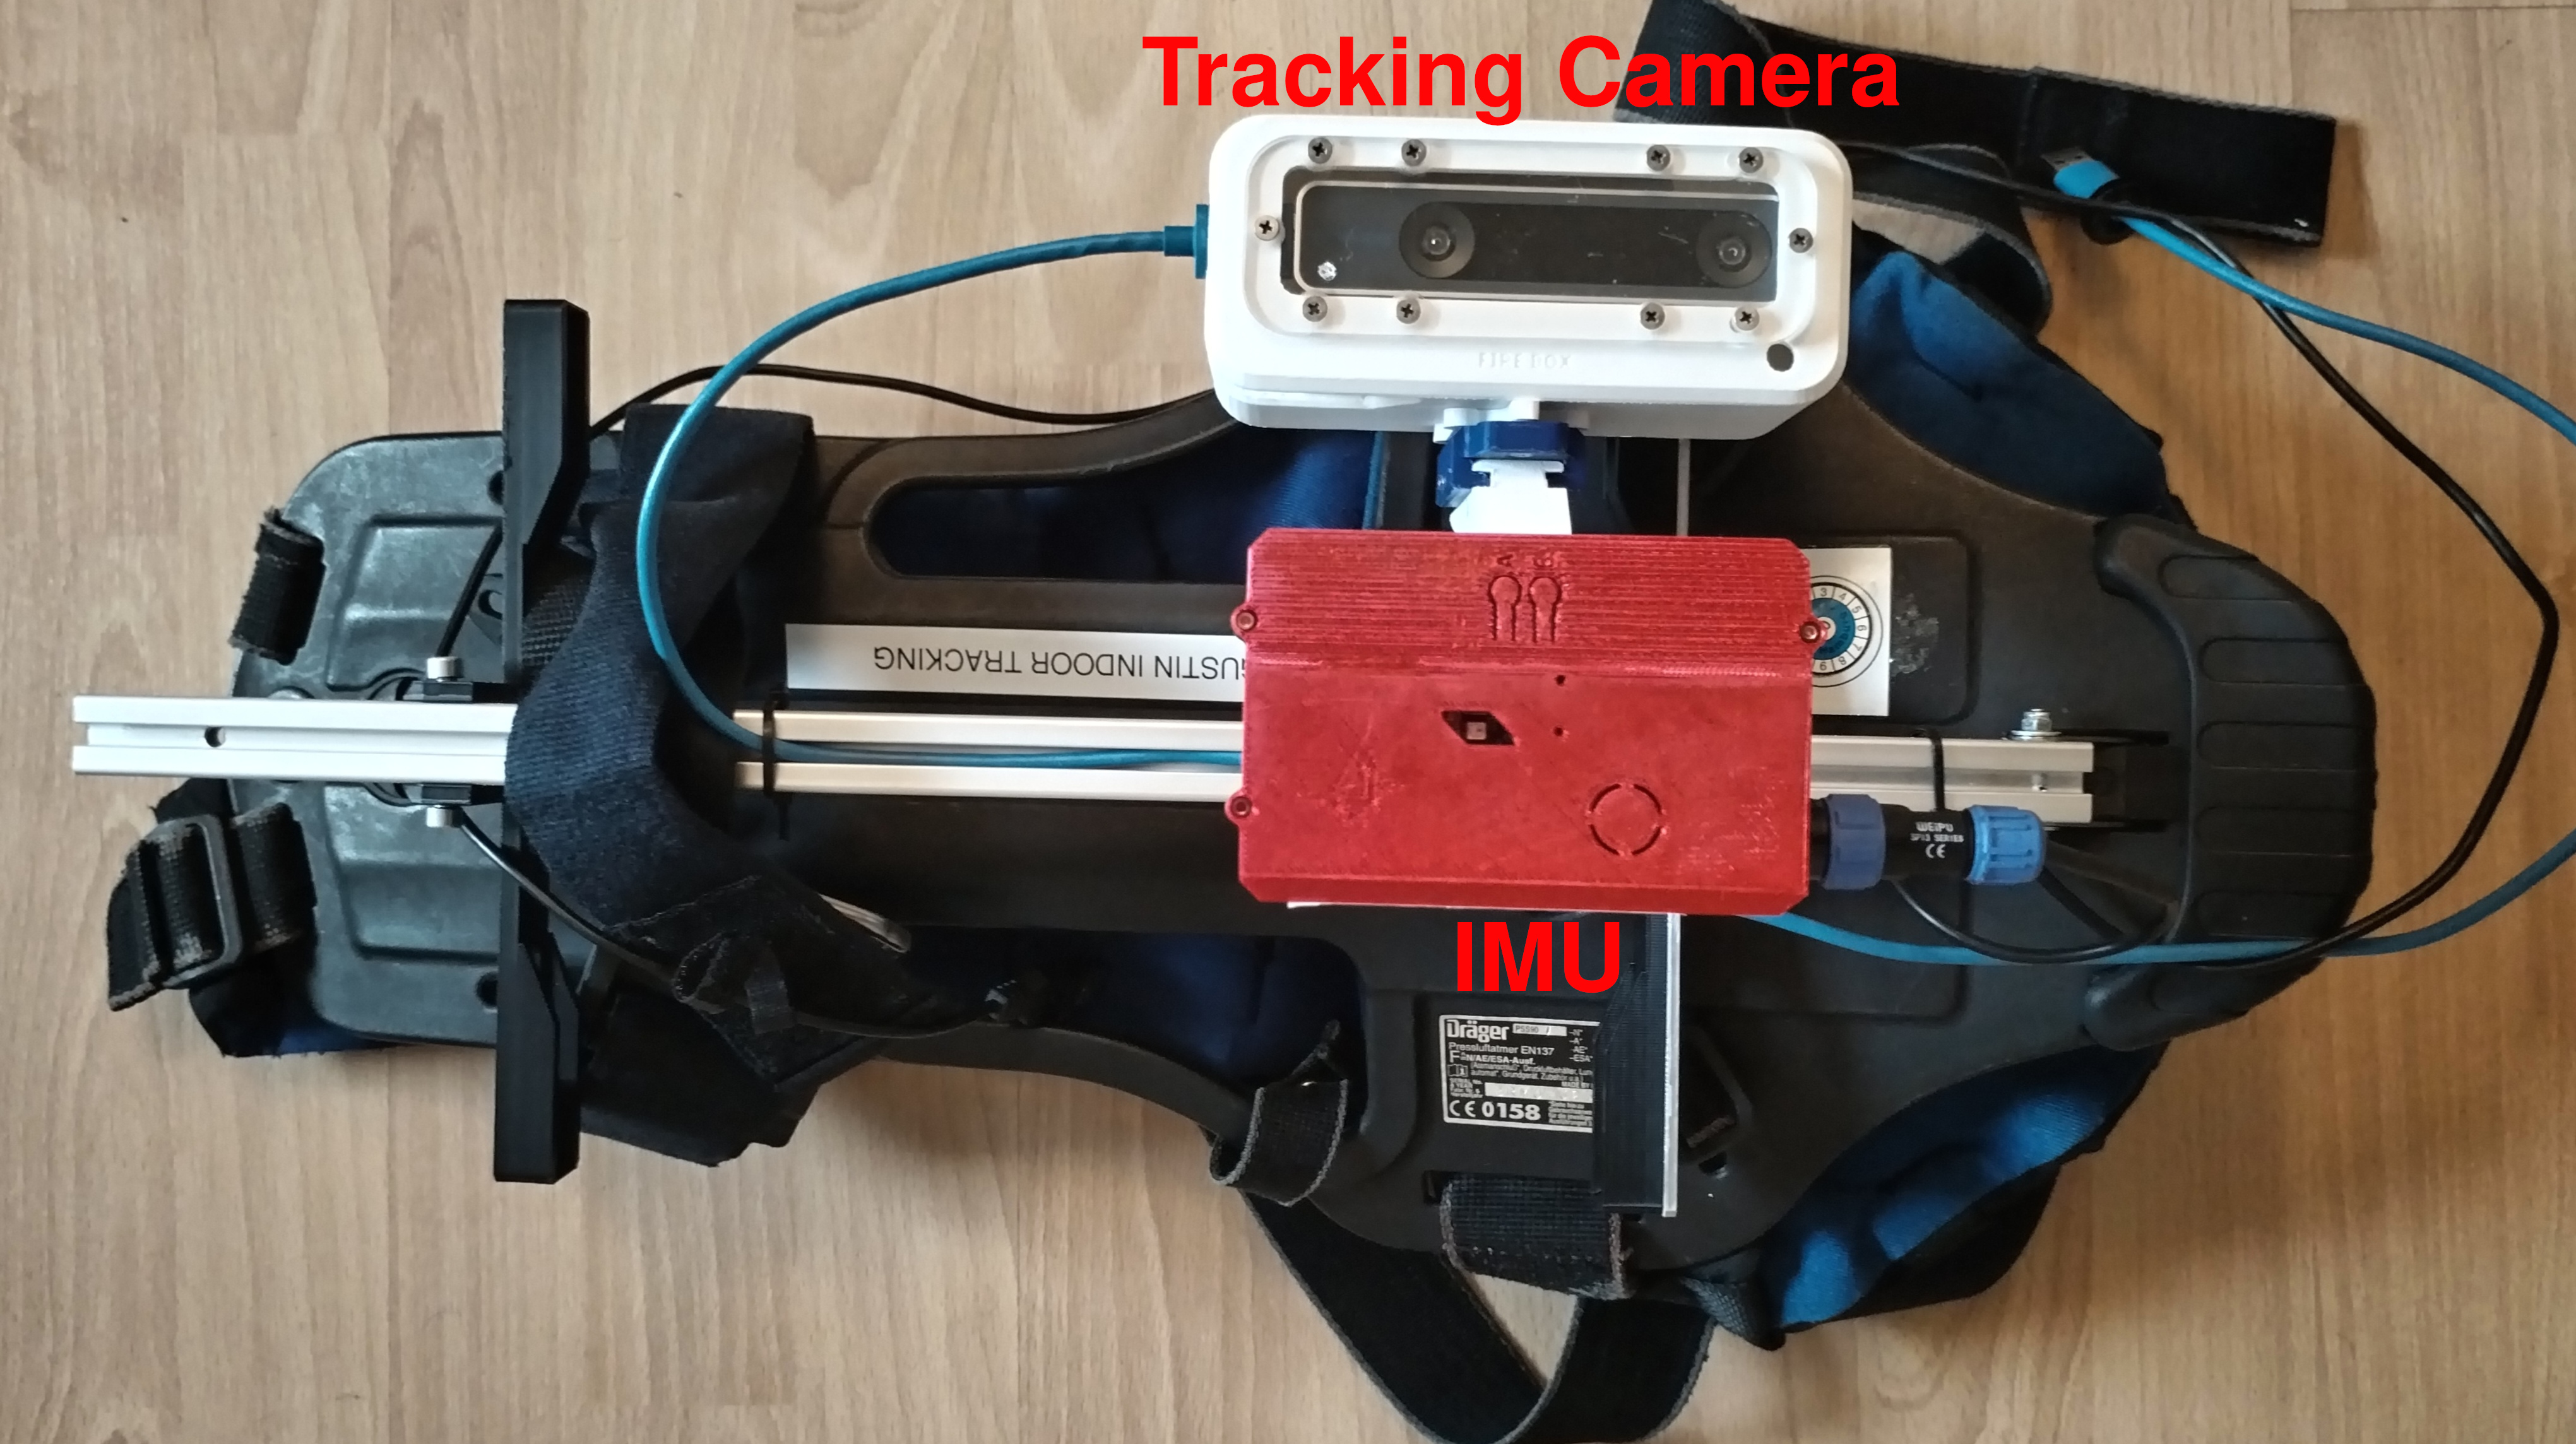
\includegraphics[width=0.6\textwidth]{Assembly.jpg}
	\caption{Sensor assembly mounted on the equipment to be worn by a firefighter.}
	\label{fig:Assembly}
\end{figure}


%%%%%%%%%%%%%%%%%%%%%%%%%%%%%%%%%%%%%%%%%%
\section{Results}
To evaluate sensor and algorithm performance, tests on a predefined path are performed. To quantify the results, the deviation from the true path is evaluated at a set of control points. The control points represent changes in heading. This allows an easy comparison between the true path and the measured path.

\subsection{Performance during Walking}

To evaluate the enhanced PDR and test the step detection during longer walking events, experiments are performed, where an individual is walking on a 33\,m long path. The position estimates of the tracking camera and the step-detection are combined in the presented sensor-date fusion algorithm.
The results show an increased accuracy of the enhanced step-detection algorithm compared to step-detection algorithms relying on peak detection and length estimation using a fixed step length. The right diagram in Figure \ref{fig:path} shows the estimated position of the estimation methods compared to the true path.

\subsection{Performance while Crouching} 

In the tests, a dynamic crouching movement often used in firefighting is used to better evaluate the step-detection and the Tracking Camera. To simulate obstruction of the tracking camera by dirt or heavy smoke, the tracking confidence is artificially reduced so that the step detection is highly favored. The path defined for the test has an overall length of 12\,m with four 90$^\circ$ turns, as shown in the left diagram in Figure \ref{fig:path}. The starting- and endpoint are identical. Ten test runs are performed where the individual completes the defined path in a crouching movement characteristic for firefighting operations. The results show an improvement in tracking accuracy when using the proposed algorithm compared to a system relying only on step-detection. Table \ref{tab1} shows the mean deviation at each control point of the different algorithms. In the case of high tracking confidence the mean deviation is lower than in cases where the tracking confidence is low, showing that the camera significantly influences the position estimate results. 
\begin{figure}
	\centering
	\begin{subfigure}[b]{0.49\textwidth}
		\centering
		\hspace{-2.5cm}
		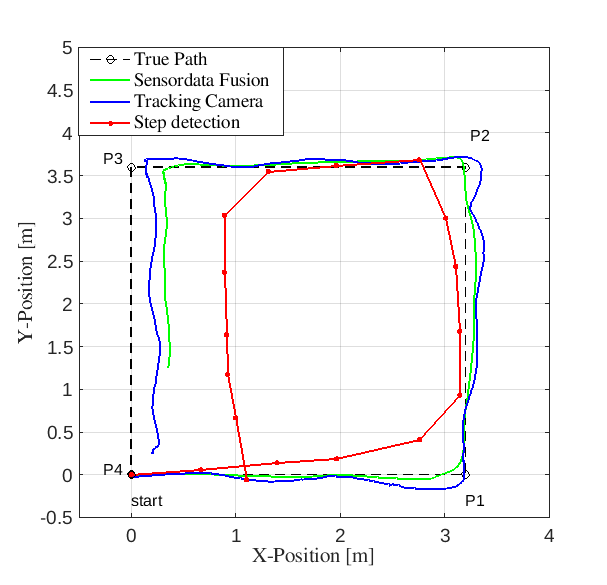
\includegraphics[width=1.11\textwidth]{Path.png}
	\end{subfigure}
	\hfill
	\begin{subfigure}[b]{0.49\textwidth}
		\centering
		\hspace{-1cm}
		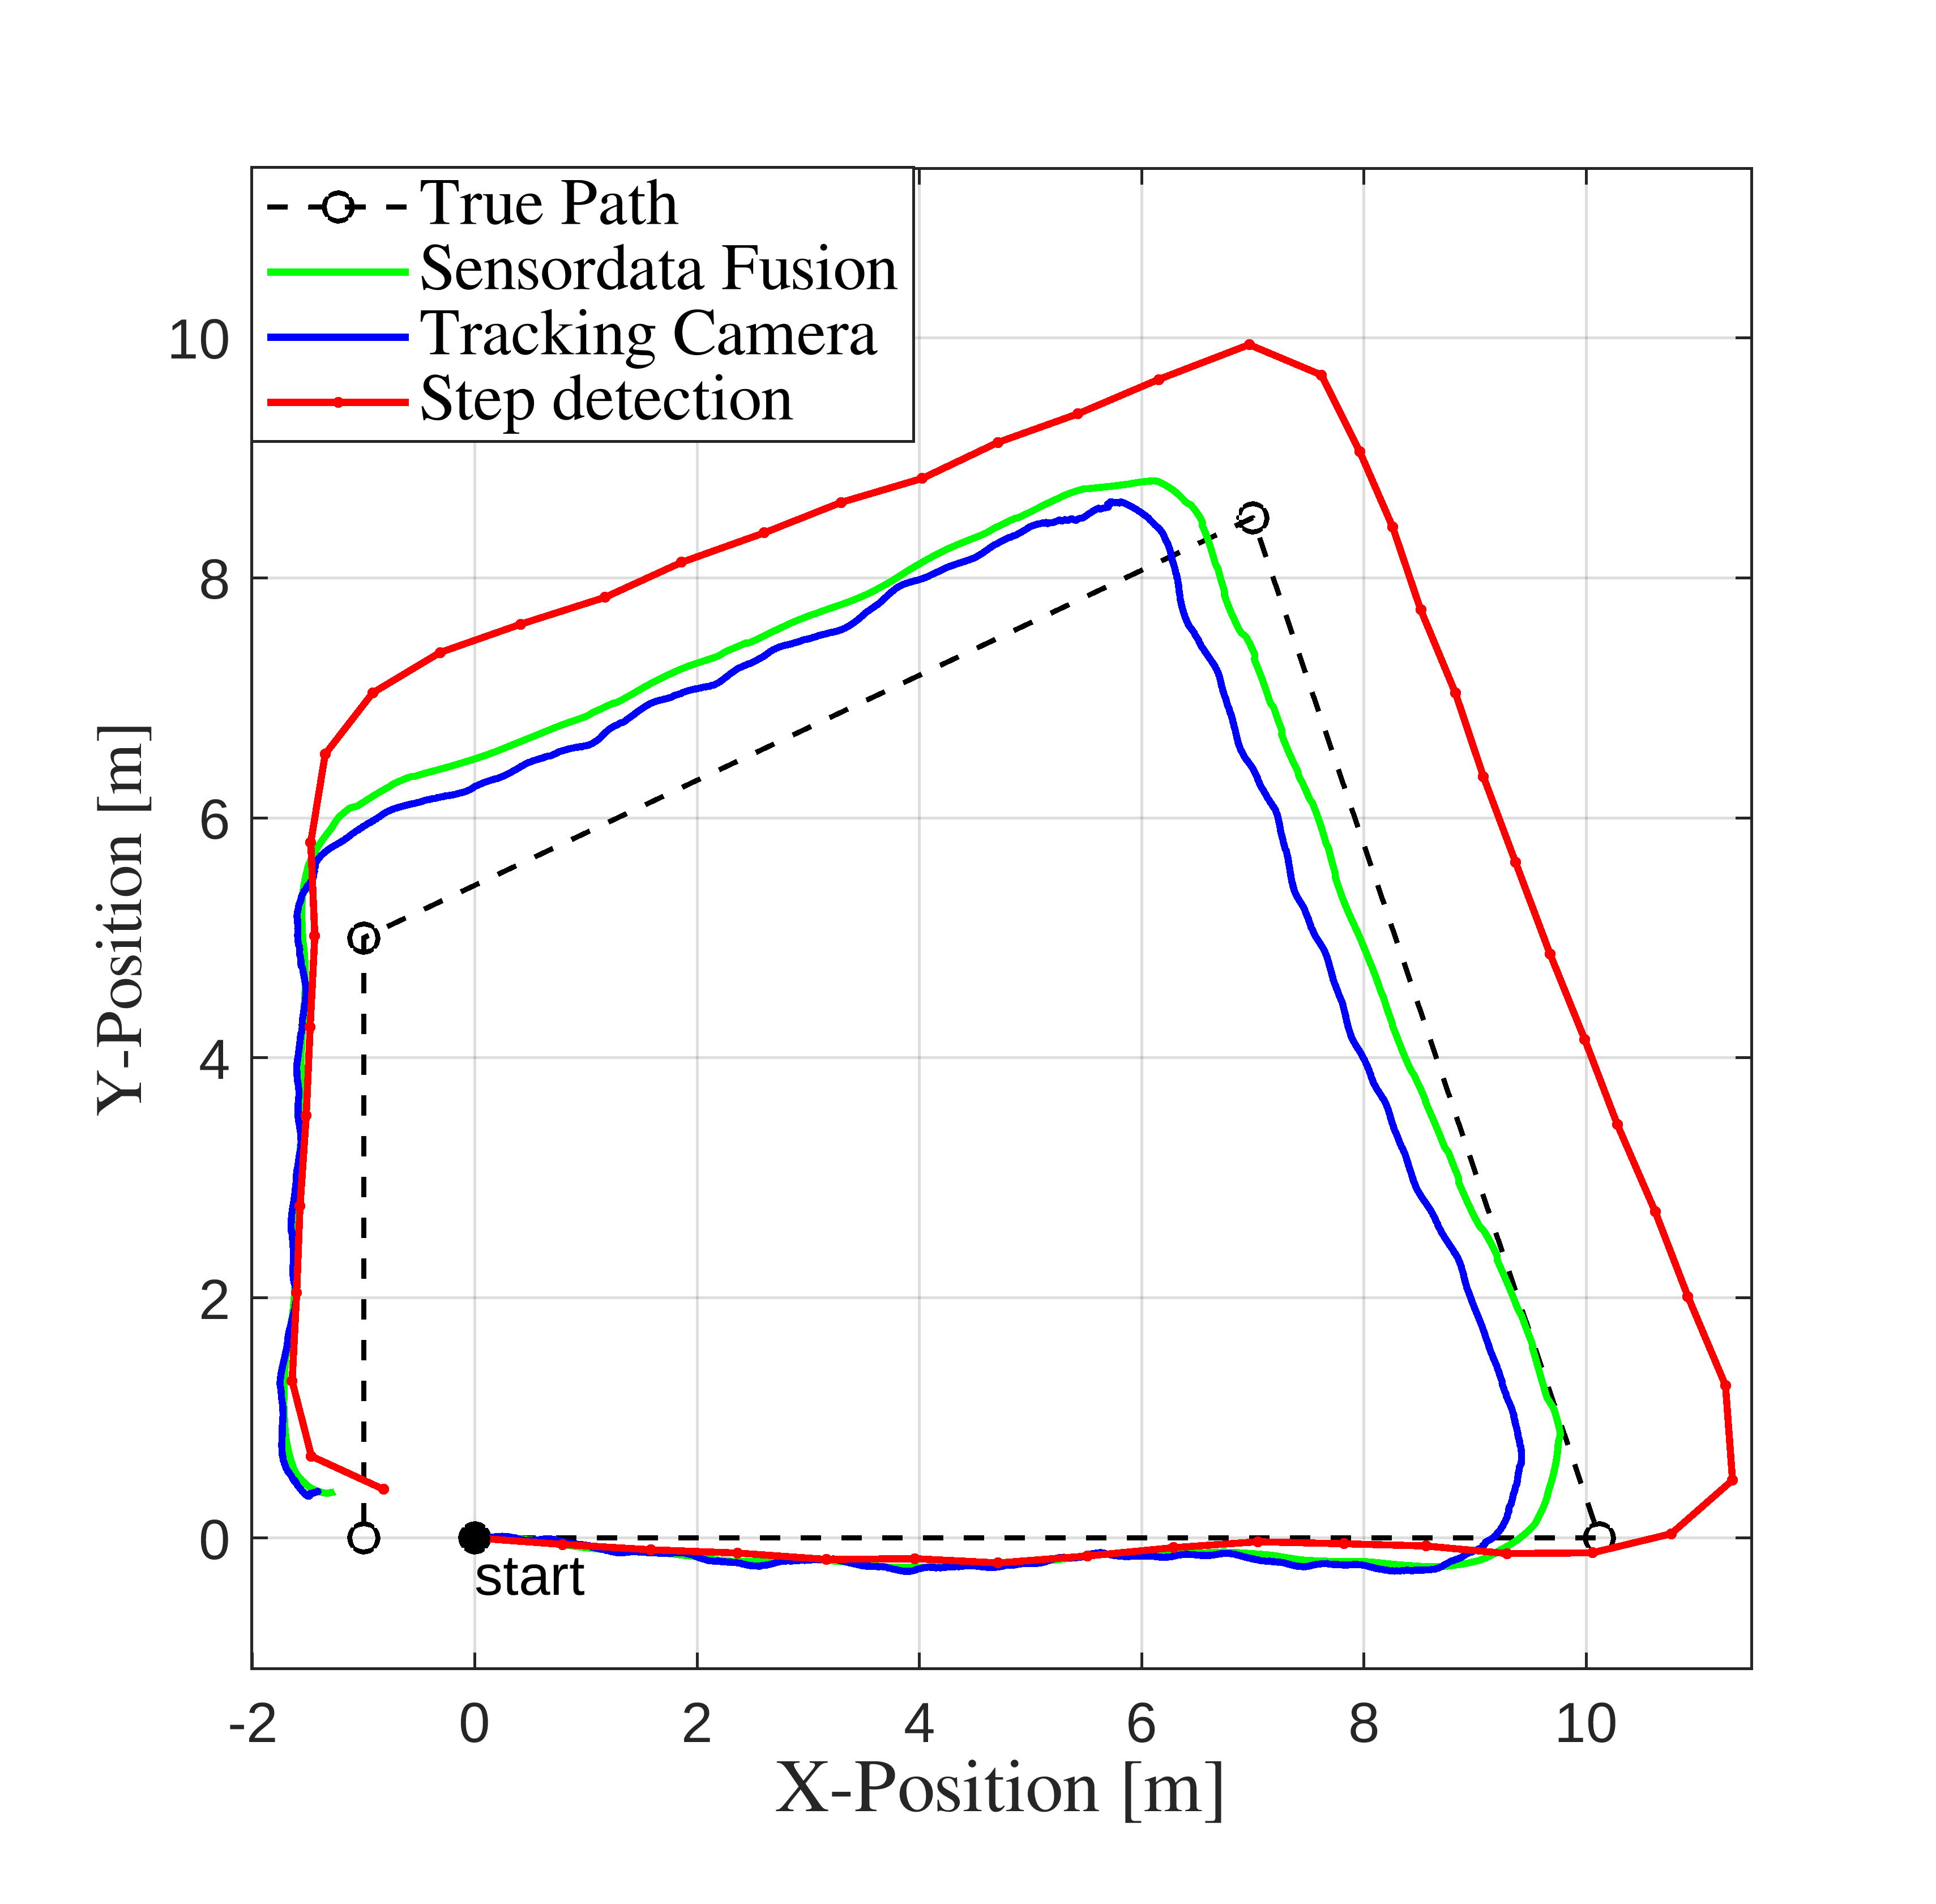
\includegraphics[width=1.1\textwidth]{Path2.png}
	\end{subfigure}
\caption{Experimental results comparing step detection only, tracking camera only, and the proposed sensor data fusion to the true path for crouching (left) and walking (right).}
\label{fig:path}
\end{figure}

\textcolor{red}{Bild (a) ist bzw war nirgends erklärt oder erwähnt. Mir ist nicht ganz klar was links und rechts ist. Ich habs mir mal zusammengereimt, bitte prüfen.}

\begin{table}[H] 
\caption{Mean deviation from the true path at four control points\label{tab1}}
\newcolumntype{C}{>{\centering\arraybackslash}X}
\begin{tabularx}{\textwidth}{lccccc}
\toprule
\textbf{Estimation Method}	& \textbf{P1}	& \textbf{P2} & \textbf{P3} & \textbf{P4} & \textbf{Mean}\\
\midrule
Step Detection	&    $1.60\mathrm{m}$ &   $2.45\mathrm{m}$ &   $2.44\mathrm{m}$  &  $1.80\mathrm{m}$ & $2.07\mathrm{m}$ \\
Sensordata Fusion  &  $0.28\mathrm{m}$  &  $0.42\mathrm{m}$  &  $0.27\mathrm{m}$ &   $0.32\mathrm{m}$ & $0.32\mathrm{m}$ \\
Sensordata Fusion (Low Tracking Confidence) &    $0.66\mathrm{m}$ &   $0.68\mathrm{m}$  &  $0.76\mathrm{m}$  &  $0.54\mathrm{m}$ & $0.66\mathrm{m}$\\
\bottomrule\\
\end{tabularx}



\end{table}






%%%%%%%%%%%%%%%%%%%%%%%%%%%%%%%%%%%%%%%%%%
\section{Conclusions}

An enhanced Pedestrian Dead Reckoning method for firefighting applications has been presented. The results of the research can be summarized as follows:
\begin{itemize}
	\item Enhancing a step-detection algorithm with a secondary sensor improves the position estimates
	\item While a tracking camera produces good position estimates and can be used as a secondary sensor, the disadvantages of a optical sensor have to be considered
	\item During more dynamic movements like crouching the system has to rely on the secondary sensor since the step-detection does not produce good position estimates
\end{itemize}
By adapting the step-detection algorithm for crouching movements the tracking estimates could be further improved. Developing a tracking camera designed for firefighting applications could also further improve position estimation.
%%%%%%%%%%%%%%%%%%%%%%%%%%%%%%%%%%%%%%%%%%
%\section{Patents}
%
%This section is not mandatory, but may be added if there are patents resulting from the work reported in this manuscript.

%%%%%%%%%%%%%%%%%%%%%%%%%%%%%%%%%%%%%%%%%%
\vspace{6pt} 

%%%%%%%%%%%%%%%%%%%%%%%%%%%%%%%%%%%%%%%%%%
%% optional
%\supplementary{The following supporting information can be downloaded at:  \linksupplementary{s1}, Figure S1: title; Table S1: title; Video S1: title.}

% Only for journal Methods and Protocols:
% If you wish to submit a video article, please do so with any other supplementary material.
% \supplementary{The following supporting information can be downloaded at: \linksupplementary{s1}, Figure S1: title; Table S1: title; Video S1: title. A supporting video article is available at doi: link.}

% Only for journal Hardware:
% If you wish to submit a video article, please do so with any other supplementary material.
% \supplementary{The following supporting information can be downloaded at: \linksupplementary{s1}, Figure S1: title; Table S1: title; Video S1: title.\vspace{6pt}\\
%\begin{tabularx}{\textwidth}{lll}
%\toprule
%\textbf{Name} & \textbf{Type} & \textbf{Description} \\
%\midrule
%S1 & Python script (.py) & Script of python source code used in XX \\
%S2 & Text (.txt) & Script of modelling code used to make Figure X \\
%S3 & Text (.txt) & Raw data from experiment X \\
%S4 & Video (.mp4) & Video demonstrating the hardware in use \\
%... & ... & ... \\
%\bottomrule
%\end{tabularx}
%}

%%%%%%%%%%%%%%%%%%%%%%%%%%%%%%%%%%%%%%%%%%

\authorcontributions{T.A.: methodology, visualisation, analysis, synthesis, testing, validation and original draft preparation. D.O.: Supervision, project management and proofreading and
	language correction All authors have read and agreed to the published version of the manuscript.}
%\authorcontributions{Conceptualization, X.X. and Y.Y.; methodology, X.X.; software, X.X.; validation, X.X., Y.Y. and Z.Z.; formal analysis, X.X.; investigation, X.X.; resources, X.X.; data curation, X.X.; writing---original draft preparation, X.X.; writing---review and editing, X.X.; visualization, X.X.; supervision, X.X.; project administration, X.X.; funding acquisition, Y.Y. All authors have read and agreed to the published version of the manuscript.}

%\funding{This research received no external funding}

%\institutionalreview{In this section, you should add the Institutional Review Board Statement and approval number, if relevant to your study. You might choose to exclude this statement if the study did not require ethical approval. Please note that the Editorial Office might ask you for further information. Please add “The study was conducted in accordance with the Declaration of Helsinki, and approved by the Institutional Review Board (or Ethics Committee) of NAME OF INSTITUTE (protocol code XXX and date of approval).” for studies involving humans. OR “The animal study protocol was approved by the Institutional Review Board (or Ethics Committee) of NAME OF INSTITUTE (protocol code XXX and date of approval).” for studies involving animals. OR “Ethical review and approval were waived for this study due to REASON (please provide a detailed justification).” OR “Not applicable” for studies not involving humans or animals.}

%\informedconsent{Any research article describing a study involving humans should contain this statement. Please add ``Informed consent was obtained from all subjects involved in the study.'' OR ``Patient consent was waived due to REASON (please provide a detailed justification).'' OR ``Not applicable'' for studies not involving humans. You might also choose to exclude this statement if the study did not involve humans.

%Written informed consent for publication must be obtained from participating patients who can be identified (including by the patients themselves). Please state ``Written informed consent has been obtained from the patient(s) to publish this paper'' if applicable.}

%\dataavailability{We encourage all authors of articles published in MDPI journals to share their research data. In this section, please provide details regarding where data supporting reported results can be found, including links to publicly archived datasets analyzed or generated during the study. Where no new data were created, or where data is unavailable due to privacy or ethical restrictions, a statement is still required. Suggested Data Availability Statements are available in section ``MDPI Research Data Policies'' at \url{https://www.mdpi.com/ethics}.} 

% Only for journal Nursing Reports
%\publicinvolvement{Please describe how the public (patients, consumers, carers) were involved in the research. Consider reporting against the GRIPP2 (Guidance for Reporting Involvement of Patients and the Public) checklist. If the public were not involved in any aspect of the research add: ``No public involvement in any aspect of this research''.}

% Only for journal Nursing Reports
%\guidelinesstandards{Please add a statement indicating which reporting guideline was used when drafting the report. For example, ``This manuscript was drafted against the XXX (the full name of reporting guidelines and citation) for XXX (type of research) research''. A complete list of reporting guidelines can be accessed via the equator network: \url{https://www.equator-network.org/}.}

%\acknowledgments{In this section you can acknowledge any support given which is not covered by the author contribution or funding sections. This may include administrative and technical support, or donations in kind (e.g., materials used for experiments).}

%\conflictsofinterest{The authors declare no conflict of interest.} 

%%%%%%%%%%%%%%%%%%%%%%%%%%%%%%%%%%%%%%%%%%
%% Optional
%\sampleavailability{Samples of the compounds ... are available from the authors.}

%% Only for journal Encyclopedia
%\entrylink{The Link to this entry published on the encyclopedia platform.}

%\abbreviations{Abbreviations}{
%The following abbreviations are used in this manuscript:\\
%
%\noindent 
%\begin{tabular}{@{}ll}
%MDPI & Multidisciplinary Digital Publishing Institute\\
%DOAJ & Directory of open access journals\\
%TLA & Three letter acronym\\
%LD & Linear dichroism
%\end{tabular}
%}

%%%%%%%%%%%%%%%%%%%%%%%%%%%%%%%%%%%%%%%%%%
%% Optional
%\appendixtitles{no} % Leave argument "no" if all appendix headings stay EMPTY (then no dot is printed after "Appendix A"). If the appendix sections contain a heading then change the argument to "yes".
%\appendixstart
%\appendix
%\section[\appendixname~\thesection]{}
%\subsection[\appendixname~\thesubsection]{}
%The appendix is an optional section that can contain details and data supplemental to the main text---for example, explanations of experimental details that would disrupt the flow of the main text but nonetheless remain crucial to understanding and reproducing the research shown; figures of replicates for experiments of which representative data are shown in the main text can be added here if brief, or as Supplementary Data. Mathematical proofs of results not central to the paper can be added as an appendix.
%
%\begin{table}[H] 
%\caption{This is a table caption.\label{tab5}}
%\newcolumntype{C}{>{\centering\arraybackslash}X}
%\begin{tabularx}{\textwidth}{CCC}
%\toprule
%\textbf{Title 1}	& \textbf{Title 2}	& \textbf{Title 3}\\
%\midrule
%Entry 1		& Data			& Data\\
%Entry 2		& Data			& Data\\
%\bottomrule
%\end{tabularx}
%\end{table}
%
%\section[\appendixname~\thesection]{}
%All appendix sections must be cited in the main text. In the appendices, Figures, Tables, etc. should be labeled, starting with ``A''---e.g., Figure A1, Figure A2, etc.

%%%%%%%%%%%%%%%%%%%%%%%%%%%%%%%%%%%%%%%%%%
\begin{adjustwidth}{-\extralength}{0cm}
%\printendnotes[custom] % Un-comment to print a list of endnotes

\reftitle{References}

% Please provide either the correct journal abbreviation (e.g. according to the “List of Title Word Abbreviations” http://www.issn.org/services/online-services/access-to-the-ltwa/) or the full name of the journal.
% Citations and References in Supplementary files are permitted provided that they also appear in the reference list here. 

%=====================================
% References, variant A: external bibliography
%=====================================
%\bibliography{bibConf}

%=====================================
% References, variant B: internal bibliography
%=====================================
\begin{thebibliography}{999}
\bibitem{arumugam2020}
Darmindra~D. Arumugam, Peter Littlewood, Nicholas Peng, and Divyam Mishra.
\newblock Long-{{Range Through-the-Wall Magnetoquasistatic Coupling}} and
{{Application}} to {{Indoor Position Sensing}}.
\newblock 19(3):507--511.

\bibitem{atemschutzunfalle.eu2023}
Atemschutzunfälle.eu.
\newblock Unfälle in {{Amerika}}.

\bibitem{caron2006}
Francois Caron, Emmanuel Duflos, Denis Pomorski, and Philippe Vanheeghe.
\newblock {{GPS}}/{{IMU}} data fusion using multisensor {{Kalman}} filtering:
Introduction of contextual aspects.
\newblock 7(2):221--230.

\bibitem{chui2009}
C.~K. Chui and G.~Chen.
\newblock {\em Kalman Filtering: With Real-Time Applications}.
\newblock {Springer}, 4th ed edition.

\bibitem{cong2023}
Li~Cong, Jingnan Tian, and Honglei Qin.
\newblock Practical {{Step Length Estimation Combining FM Radio Signal}} and
{{Accelerometer}}.
\newblock 72:1--13.

\bibitem{hajati2021}
N.~Hajati and A.~Rezaeizadeh.
\newblock A {{Wearable Pedestrian Localization}} and {{Gait Identification
		System Using Kalman Filtered Inertial Data}}.
\newblock 70.
\newblock Cited By :13.

\bibitem{hou2021}
X.~Hou and J.~Bergmann.
\newblock Pedestrian {{Dead Reckoning}} with {{Wearable Sensors}}: {{A
		Systematic Review}}.
\newblock 21(1):143--152.
\newblock Cited By :52.

\bibitem{jen2023}
Y.-H. Jen, C.-H. Huang, S.~Tsai, and K.-W. Chiang.
\newblock A {{MULTI-IMU BASED SELF-CONTAINED PEDESTRIAN NAVIGATION ALGORITHM}}.
\newblock XLVIII-1/W1-2023:603--608.
\newblock Multiple IMUs improve heading estimatioon,.

\bibitem{lu2019}
C.~Lu, H.~Uchiyama, D.~Thomas, A.~Shimada, and R.-I. Taniguchi.
\newblock Indoor positioning system based on chest-mounted {{IMU}}.
\newblock 19(2).
\newblock Cited By :47.

\bibitem{petukhov2022}
Nikita~I. Petukhov, Vladimir~N. Zamolodchikov, Alexander~P. Malyshev,
Tatyana~A. Brovko, Sergey~A. Serov, and Ilya~V. Korogodin.
\newblock Synthesis of {{PDR Algorithm}} and {{Experimental Estimation}} of
{{Accuracy}} of {{Step Length Estimation Methods}}.
\newblock In {\em 2022 4th {{International Youth Conference}} on {{Radio
			Electronics}}, {{Electrical}} and {{Power Engineering}} ({{REEPE}})}, pages
1--5. {IEEE}.

\bibitem{sadruddin2020}
Hamza Sadruddin, Ahmed Mahmoud, and Mohamed~M. Atia.
\newblock Enhancing {{Body-Mounted LiDAR SLAM}} using an {{IMU-based Pedestrian
		Dead Reckoning}} ({{PDR}}) {{Model}}.
\newblock In {\em 2020 {{IEEE}} 63rd {{International Midwest Symposium}} on
	{{Circuits}} and {{Systems}} ({{MWSCAS}})}, pages 901--904.

\bibitem{nistsematech2012}
NIST SEMATECH.
\newblock {{NIST}}/{{SEMATECH}} e-{{Handbook}} of {{Statistical Methods}}.

\bibitem{shin2007}
S.~H. Shin, C.~G. Park, J.~W. Kim, H.~S. Hong, and J.~M. Lee.
\newblock Adaptive {{Step Length Estimation Algorithm Using Low-Cost MEMS
		Inertial Sensors}}.
\newblock In {\em 2007 {{IEEE Sensors Applications Symposium}}}, pages 1--5.

\bibitem{wang2016}
Qu~Wang, Haiyong Luo, Fang Zhao, and Wenhua Shao.
\newblock An indoor self-localization algorithm using the calibration of the
online magnetic fingerprints and indoor landmarks.
\newblock In {\em 2016 {{International Conference}} on {{Indoor Positioning}}
	and {{Indoor Navigation}} ({{IPIN}})}, pages 1--8.

\bibitem{weinberg2002}
Harvey Weinberg.
\newblock Using the {{ADXL202}} in {{Pedometer}} and {{Personal Navigation
		Applications}}.

\bibitem{wu2022}
Yibin Wu, Jian Kuang, and Xiaoji Niu.
\newblock Wheel-{{INS2}}: {{Multiple MEMS IMU-based Dead Reckoning System}} for
{{Wheeled Robots}} with {{Evaluation}} of {{Different IMU Configurations}}.
\newblock Comment: Accepted to IEEE Transactions on Intelligent Transportation
Systems.

\bibitem{zaarane2020}
Abdelmoghit Zaarane, Ibtissam Slimani, Wahban Al~Okaishi, Issam Atouf, and
Abdellatif Hamdoun.
\newblock Distance measurement system for autonomous vehicles using stereo
camera.
\newblock 5:100016.

\bibitem{zhao2021}
Tianyi Zhao and Mohammed~Jalal Ahamed.
\newblock Pseudo-{{Zero Velocity Re-Detection Double Threshold Zero-Velocity
		Update}} ({{ZUPT}}) for {{Inertial Sensor-Based Pedestrian Navigation}}.
\newblock 21(12):13772--13785.

\bibitem{zhao2022}
Yue Zhao, Jianyong Wang, and Chengyong Duan.
\newblock Design and application research of mine underground disaster relief
personnel positioning system based on {{MEMS}} sensor.
\newblock In {\em International {{Conference}} on {{Neural Networks}},
	{{Information}}, and {{Communication Engineering}} ({{NNICE}} 2022)}, volume
12258, pages 695--704. {SPIE}.

\bibitem{zizzo2017}
Giulio Zizzo and Lei Ren.
\newblock Position {{Tracking During Human Walking Using}} an {{Integrated
		Wearable Sensing System}}.
\newblock 17(12):2866.
\end{thebibliography}

% If authors have biography, please use the format below
%\section*{Short Biography of Authors}
%\bio
%{\raisebox{-0.35cm}{\includegraphics[width=3.5cm,height=5.3cm,clip,keepaspectratio]{Definitions/author1.pdf}}}
%{\textbf{Firstname Lastname} Biography of first author}
%
%\bio
%{\raisebox{-0.35cm}{\includegraphics[width=3.5cm,height=5.3cm,clip,keepaspectratio]{Definitions/author2.jpg}}}
%{\textbf{Firstname Lastname} Biography of second author}

% For the MDPI journals use author-date citation, please follow the formatting guidelines on http://www.mdpi.com/authors/references
% To cite two works by the same author: \citeauthor{ref-journal-1a} (\citeyear{ref-journal-1a}, \citeyear{ref-journal-1b}). This produces: Whittaker (1967, 1975)
% To cite two works by the same author with specific pages: \citeauthor{ref-journal-3a} (\citeyear{ref-journal-3a}, p. 328; \citeyear{ref-journal-3b}, p.475). This produces: Wong (1999, p. 328; 2000, p. 475)

%%%%%%%%%%%%%%%%%%%%%%%%%%%%%%%%%%%%%%%%%%
%% for journal Sci
%\reviewreports{\\
%Reviewer 1 comments and authors’ response\\
%Reviewer 2 comments and authors’ response\\
%Reviewer 3 comments and authors’ response
%}
%%%%%%%%%%%%%%%%%%%%%%%%%%%%%%%%%%%%%%%%%%
%\PublishersNote{}
\end{adjustwidth}
\end{document}

